\chapter{Theoretical Background}
\label{chap:theoretical-background}
Since the application's core is sentiment analysis, it is necessary to define the basic concepts. \textcolor{lightgray}{Lorem ipsum dolor sit amet, consectetur adipiscing elit. Sed non risus. Suspendisse lectus tortor, dignissim sit amet, adipiscing nec, ultricies sed, dolor. Lorem ipsum dolor sit amet, consectetur adipiscing elit. Sed non risus. Suspendisse lectus tortor, dignissim sit amet, adipiscing nec, ultricies sed, dolor. Lorem ipsum dolor sit amet, consectetur adipiscing elit. Sed non risus. Suspendisse lectus tortor, dignissim sit amet, adipiscing nec, ultricies sed, dolor. Lorem ipsum dolor sit amet, consectetur adipiscing elit. Sed non risus.}

\section{Sentiment Analysis Basics}
\label{sec:sentiment-analysis-basics}
Sentiment analysis or opinion mining is a subfield of \acrshort{nlp} that aims to identify and extract opinions and emotions from a text. The goal is to determine the author's attitude towards a particular topic or the overall contextual polarity~of various document levels. We measure the text's polarity using a numerical scale ranging from -1 to 1. The low-end score of the scale signifies a negative sentiment, zero represents neutrality, and the high-end score indicates a positive sentiment. This scale effectively estimates the degree of negativity or positivity in the text's tone. 

The extraction of opinions and emotions has applications in various areas, from product reviews to political events. Hence, it is imperative to work in different domains (see \cite{PIRYANI2017122}). Because of cross-domain and cross-language, two of the most general issues in sentiment analysis, this thesis will focus only on the financial domain in English. Nevertheless, domain-specific sentiment analysis achieves remarkable accuracy while staying highly domain-sensitive, as shown \cite{saunders_2020}. To delve deeper into cross issues, \citeauthor{liu2022sentiment} provides further details in his book \citetitle{liu2022sentiment}\todo{(Q-1.1) Zeptat se - nebo je lepší odkaz "in his work Lei, 2022" v context citatce v Bibliography, kde odkazuji na konkrétní strany z jeho knihy, které se daným problémem odkazují.}.

\subsection{Levels of Sentiment Analysis}
\label{subsec:levels-of-sentiment-analysis}
Sentiment analysis has been studied at several levels of granularity: Document-level, Sentence-level, Phrase-level, and Entity-level\footnote{Entities are sometimes referred to as targets, hence Target-level or Target-based sentiment analysis.}, as illustrated in Fig. \ref{fig:sa-levels}.

\begin{figure}[H]
    \centering
    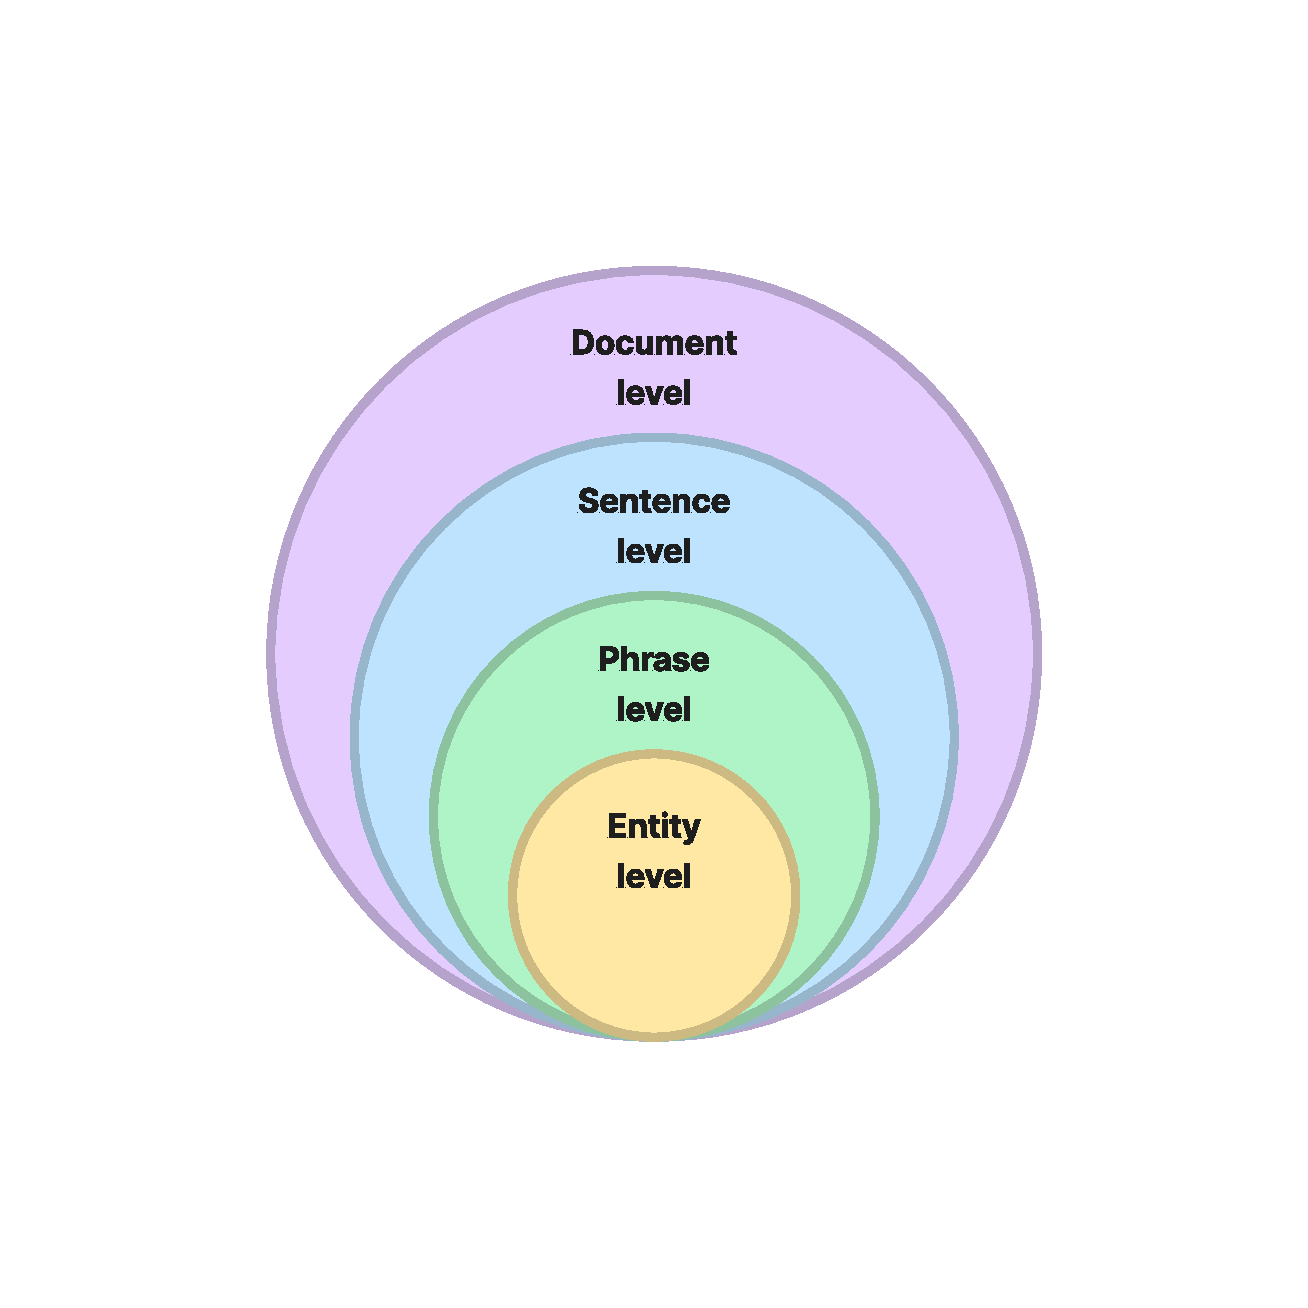
\includegraphics[width=0.5\textwidth]{img/sa-levels.pdf}
    \caption{Levels of sentiment analysis (inspired by \cite{Wankhade2022}).}
    \label{fig:sa-levels}
\end{figure}
\todo{(Q-1.1.1-1) Zeptat se - Je třeba citovat?}

\subsubsection*{Document-level}
\label{subsubsec:document-level}
%At the first level is document-level sentiment analysis. This level is the most straight.
Document-level sentiment analysis is the most straight level. The task is to determine the overall emotional context of the entire document, such as a chapter, article, or review, whether or not involving a study of entities or aspects. This level gives us a general assessment of whether the content is more likely to be positive, negative, or neutral. 

\subsubsection*{Sentence-level}
\label{subsubsec:sentence-level}
Sentiment analysis at the sentence level focuses on individual sentences within the text. We observe the polarity of each sentence autonomously, employing the same methodologies utilized at the document level but with an increased volume of training data and enhanced processing resources. This level is more challenging than the document level because it requires a more in-depth understanding of the text. 

\subsubsection*{Phrase-level}
\label{subsubsec:phrase-level}
Phrase-level sentiment analysis examines sentiment within smaller linguistic units such as phrases or sentence members. Thus, it can better reveal the emotional charge in specific parts of sentences.  Additionally, this level is more challenging than the sentence level because it requires a more detailed understanding of the text. 


\subsubsection*{Entity-level}
\label{subsubsec:entity-level}
The most elaborative level is entity-level sentiment analysis, where we study sentiment associated with specific entities mentioned in the text. This level provides a detailed look at the expressed polarity of certain products, individuals, or organizations. One of the main tasks in this scope is the named entity recognition, which will be discussed later.

\paragraph{}

Some researchers classify the last level as the aspect-level, as noted by \cite{Wankhade2022}, or a more detailed entity-level version called the feature-level proposed by \cite{Jenifer2017}. While both approaches aim to evaluate sentiment towards specific aspects, they differ in their task approach. Relationships between these levels are illustrated in Fig. \ref{fig:enity-feature-aspect-level}.

In the first case, aspects are considered without directly mentioning entities in the text. We are not interested in the entities since the \todo{(Q-1.1.1-2) Zeptat se - Nebo zaměnit "investigated textual data" za "(input) data"?} investigated textual data are commonly associated with them\footnote{Entities are not handled in this case, but we provide them here for a better understanding.}, such as reviews. The study conducted by \cites{Wang2019} analyzed sentiment at the aspect level within restaurant reviews. It primarily examines aspects such as food, price, service, and others. In~the feature-based approach, aspects are commonly associated with an entity's features by connecting the entity and its aspects in text. To illustrate, consider the sentence:\begin{quote}
    \textit{``The battery life of this phone is excellent, but the camera is not good.''}
\end{quote} At the feature level, we identify \textit{the battery life} and \textit{camera} as specific features of entity \textit{the phone}, allowing us to determine the polarity of each entity's feature.

\begin{figure}[H]
    \centering
    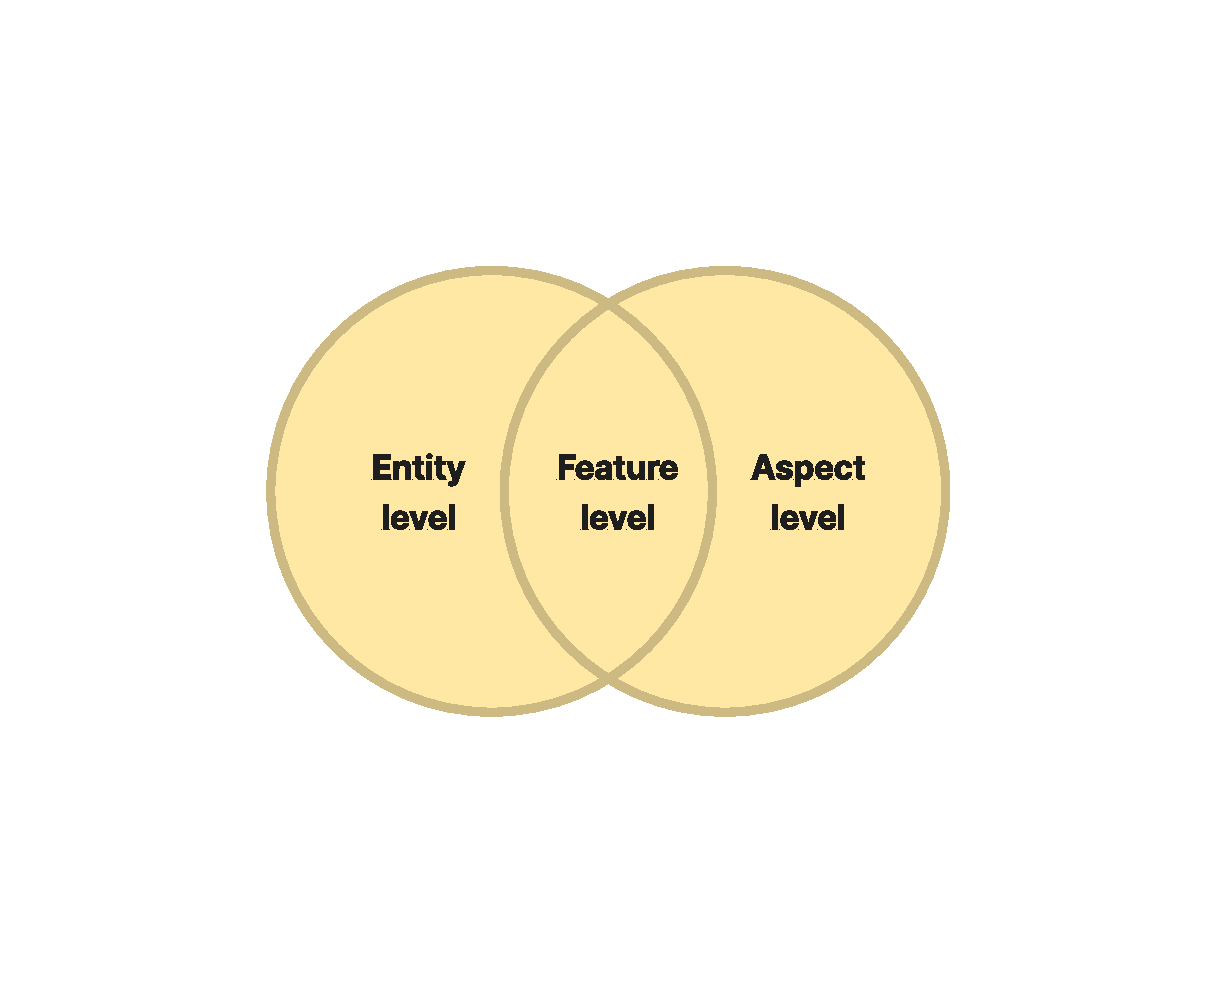
\includegraphics[width=0.5\textwidth]{img/entity-feature-aspect-level.pdf}
    \caption{Comprehensive overview of the last level.}
    \label{fig:enity-feature-aspect-level}
\end{figure}

% Každé rozdělení posledního levelu zkoumáme v rámci předešlých levelů. Toz namneá, že entity level zkoumáme v rámci document, sentence a nebo phrase. Opačně můžeme ale i nemusíme zkoumat document, sentence a nebo phrase v rámci entity levelu.

The term entity-level sentiment analysis is frequently employed in literature, and some studies consider it synonymous with targeted sentiment analysis, \linebreak as discussed \cite{ronningstad-etal-2022-entity} in the terminology review. For our purposes, entity-level sentiment analysis better captures the aggregate, document-wide approach, where a single entity can be associated with multiple targets in different sentences, discerning it from traditional target-level sentiment analysis. 

However, this thesis primarily focuses on entity-level sentiment analysis, excluding consideration of the entity's features. This decision is motivated by treating the mentioned companies in news articles as entities rather than delving into their specific aspects.\todo{TODO: Pokud nenarazím na článek, který by to vyvrátil. Navíc se zkoumáním aspektů by přibylo spousty práce.} Additionally, entity and aspect extraction as separate tasks are complex and challenging, given that the methods \textcolor{lightgray}{and facets} employed for recognition differ due to their distinct characteristics \parencite{Liu2015, Zhang2014}. 

\subsection{Workflow of Sentiment Analysis}
\label{subsec:workflow-of-sentiment-analysis}
The sentiment analysis process can be divided into three main steps: data retrieval, preprocessing, and analysis. The following sections will discuss these steps in more detail.

\section{Named Entity Recognition}
\label{sec:named-entity-recognition}
We will focus on the named entity recognition, also known as entity extraction, in the context of news. 
% Good survey https://wandb.ai/madhana/Named_Entity_Recognition/reports/A-Beginner-s-Guide-to-Named-Entity-Recognition-NER---VmlldzozNjE2MzI1
Named entity recognition is a subtask of \acrshort{nlp} with a focus on identifying and classifying named entities in text into predefined categories such as the names of organizations, persons, locations, expressions of times, quantities, monetary values, and so on. Named entity recognition is a crucial step in entity-level sentiment analysis, as it allows us to identify the sentiment associated with specific entities mentioned in the text. \textcolor{lightgray}{And so on...} %In a given text, there could be several mentions of separate entities, each possibly referred to directly and indirectly multiple times, with varying polarities.

\section{Time Series Forecasting Integration}
\label{sec:integration-with-time-series-forecasting-for-market-trends}
We will focus on integrating time series forecasting in the context of news.

\todo{(Q-1.3) Zeptat se - Bude třeba úvod do stock marketu? Podle mě ne a zbytečně by se to míchalo do (technology) teoretického pozadí.}